\documentclass[11pt]{standalone}
\usepackage{amssymb}
\usepackage{amsmath}
\usepackage[no-math]{fontspec}
\usepackage{unicode-math}
\usepackage{libertinus}
\usepackage{pgf,xcolor}
\usepackage{tikz}
\usetikzlibrary{arrows.meta, backgrounds}
\usepackage{pgfplots}
\pgfplotsset{compat=newest}

\definecolor{my_darkgray}{HTML}{484949}
\definecolor{my_lightgray}{HTML}{F3F4F4}
\definecolor{my_darkblue}{HTML}{005A94}
\definecolor{my_lightblue}{HTML}{CCDEE9}
\definecolor{my_yellow}{HTML}{FFEC7F}
\definecolor{my_red}{HTML}{E60000}
\definecolor{my_orange}{HTML}{E87846}

\begin{document}
% ---------------------------------------------------------------
%  Entscheidungsweg fuer lineare DGL 1. Ordnung: erst die homogene
%  Loesung, dann die Wahl des Verfahrens fuer die partikulaere
%  Loesung, am Ende y = y_h + y_p.
%  Koordinaten explizit gesetzt (keine positioning-Bibliothek,
%  damit die Praeambel unveraendert bleibt).
% ---------------------------------------------------------------
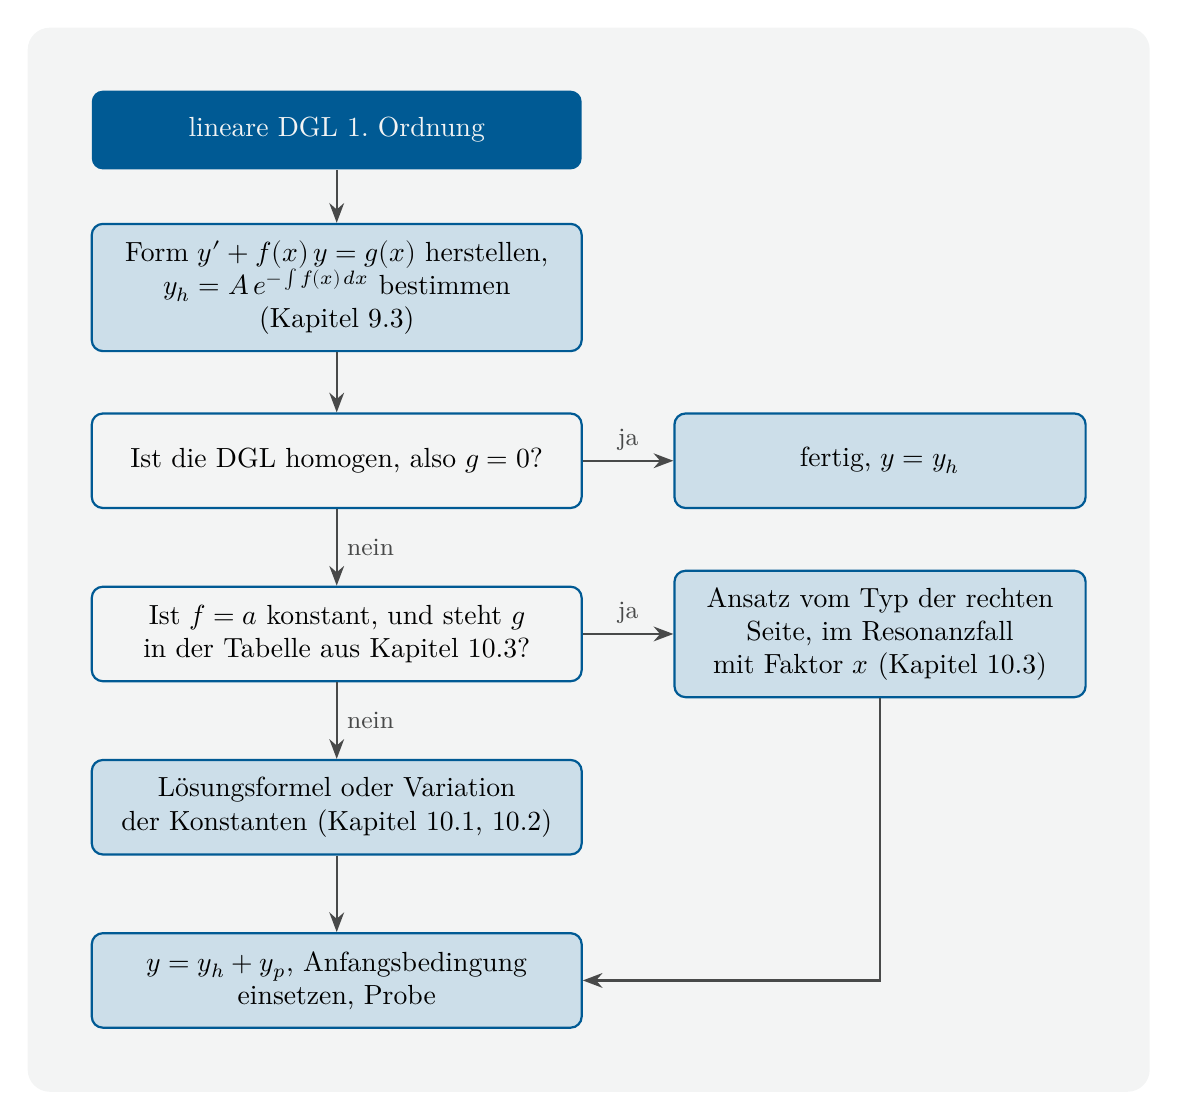
\begin{tikzpicture}[
    show background rectangle,
    background rectangle/.style={fill=my_lightgray, rounded corners=8pt},
    inner frame sep=0.8cm,
    start/.style={fill=my_darkblue, text=my_lightgray, rounded corners=4pt,
        text width=5.8cm, align=flush center, inner sep=6pt, minimum height=1cm},
    frage/.style={draw=my_darkblue, thick, rounded corners=4pt,
        text width=5.8cm, align=flush center, inner sep=6pt, minimum height=1.2cm},
    verfahren/.style={draw=my_darkblue, thick, fill=my_lightblue,
        rounded corners=4pt, text width=4.8cm, align=flush center, inner sep=6pt,
        minimum height=1.2cm},
    schritt/.style={draw=my_darkblue, thick, fill=my_lightblue,
        rounded corners=4pt, text width=5.8cm, align=flush center, inner sep=6pt,
        minimum height=1.2cm},
    pfeil/.style={-{Stealth[length=2.5mm]}, thick, my_darkgray},
    marke/.style={font=\small, text=my_darkgray},
]
\node[start] (s) at (0, 0) {lineare DGL 1.~Ordnung};

\node[schritt] (h) at (0, -2)
    {Form $y' + f(x)\,y = g(x)$ herstellen,\\
     $y_h = A\,e^{-\int f(x)\,dx}$ bestimmen\\ (Kapitel 9.3)};

\node[frage] (q1) at (0, -4.2) {Ist die DGL homogen, also $g = 0$?};
\node[verfahren] (m1) at (6.9, -4.2) {fertig, $y = y_h$};

\node[frage] (q2) at (0, -6.4)
    {Ist $f = a$ konstant, und steht $g$\\ in der Tabelle aus Kapitel 10.3?};
\node[verfahren] (m2) at (6.9, -6.4)
    {Ansatz vom Typ der rechten\\ Seite, im Resonanzfall\\
     mit Faktor $x$ (Kapitel 10.3)};

\node[schritt] (m3) at (0, -8.6)
    {Lösungsformel oder Variation\\ der Konstanten (Kapitel 10.1, 10.2)};

\node[schritt] (z) at (0, -10.8)
    {$y = y_h + y_p$, Anfangsbedingung\\ einsetzen, Probe};

\draw[pfeil] (s) -- (h);
\draw[pfeil] (h) -- (q1);
\draw[pfeil] (q1) -- node[marke, above] {ja} (m1);
\draw[pfeil] (q1) -- node[marke, right] {nein} (q2);
\draw[pfeil] (q2) -- node[marke, above] {ja} (m2);
\draw[pfeil] (q2) -- node[marke, right] {nein} (m3);
\draw[pfeil] (m3) -- (z);
\draw[pfeil] (m2.south) |- (z.east);
\end{tikzpicture}
\end{document}
